Con la presente il gruppo Merl intende comunicarvi che si impegnerà a finire il progetto didattico entro il giorno 7 Maggio 2022.

Dopo un’attenta discussione siamo riusciti a elaborare un preventivo relativo al capitolato C5 Login Warrior dell’azienda Zucchetti S.p.A.. La seguente tabella riesce a spiegare al meglio le ore di lavoro dei vari ruoli che si occupano del progetto e dei loro relativi costi.

\begin{center}
  \begin{tabular}{ |l|c|c|c|c| }
    \hline
                   & Ore & Ore Totali & Costo (€) & Costo Totale (€) \\
    \hline
    Responsabile   & 9   & 63         & 30        & 1890             \\
    \hline
    Amministratore & 8   & 56         & 20        & 1120             \\
    \hline
    Analista       & 5   & 35         & 25        & 875              \\
    \hline
    Progettista    & 23  & 161        & 25        & 4025             \\
    \hline
    Programmatore  & 24  & 168        & 15        & 2520             \\
    \hline
    Verificatore   & 26  & 182        & 15        & 2730             \\
    \hline
  \end{tabular}
\end{center}

Ecco anche un grafico che rappresenta la percentuale di lavoro di ciascun ruolo:
\begin{center}
  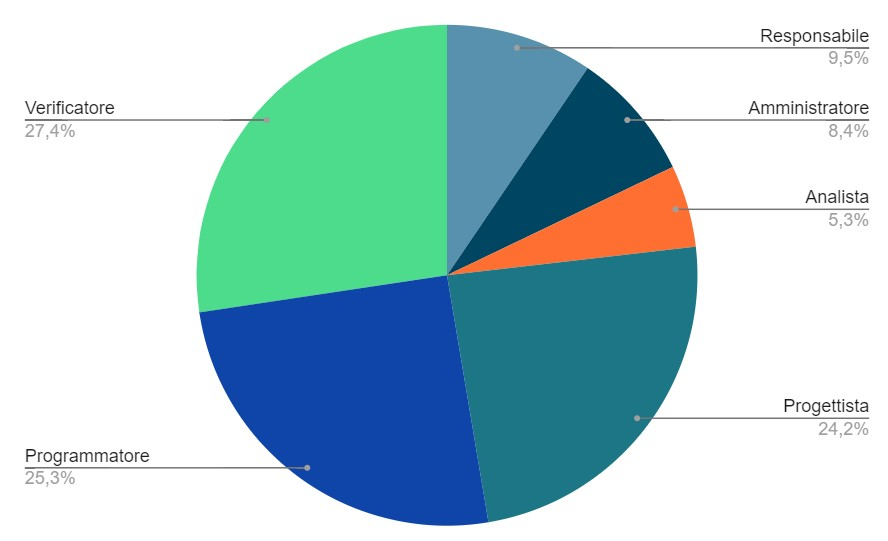
\includegraphics[width=1.0\textwidth]{percentuale_ore}
\end{center}

Il costo finale calcolato in base alle tariffe orarie dei ruoli e alle ore preventivate risulta di :
\textbf{€ 13160}.

In totale il monte ore è pari a \textbf{665 ore}, esplicando quindi \textbf{95 ore a testa} per ciascun membro del gruppo.
